\chapter{Probability basics}\label{ch:prob}
\index{probability}\index{expected value}\index{linearity of expectation}\index{Bayes' theorem}\index{coupon collector}\index{indicator variable}

Contest probability problems look continuous but almost never
are: every die, card, robot step, or random index is a finite
uniform draw, so every question is counting in disguise --- or
expectation, which is counting with weights. This chapter
teaches the three tools that solve the whole CSES probability
set: enumerate outcomes exactly with dynamic programming, take
expectation apart with linearity (which never requires
independence), and condition correctly with Bayes' rule. After
it you will know when a problem wants an exact rational answer,
when it wants a recurrence, and why reaching for a random-number
generator is usually the wrong move.

\emph{This chapter is optional for the core route; it feeds the
CSES ``Probability'' problem set and a small but real slice of
Codeforces and USACO-G.}

% from-zero:begin
\begin{rulebox}[Before you start]
Chapter~14 (modular arithmetic) and \textbf{Book~2, Chapter~12} (probability on finite spaces). \emph{Recap:} on a finite sample space with equally likely outcomes, $P(A)=|A|/|\Omega|$: probability is counting.
\begin{itemize}
\item The expected value of a random quantity is the average you would see over many repetitions.
\end{itemize}
\end{rulebox}
\begin{wins}[After this chapter you can]
\begin{itemize}
\item turn a ``probability that\dots'' problem into a counting problem;
\item compute an expected value with linearity of expectation, without listing outcomes;
\item apply conditional probability and Bayes' rule to a short word problem;
\item compute a probability exactly with DP and know when to settle for simulation.
\end{itemize}
\end{wins}
\begin{principle}[How to think about this]
Do not memorise probability formulas. Picture the experiment as a list of equally likely outcomes and count the ones you want. When counting directly is painful, switch viewpoints: expected values add up even when events are tangled together, so break the quantity into small indicator pieces and add their expectations.
\end{principle}
% from-zero:end

\section{Finite probability: counting in disguise}\label{sec:finite}
\index{sample space}\index{event}\index{complement rule}
On a finite \emph{sample space} $\Omega$ with equally likely
outcomes, $\Pr[A]=|A|/|\Omega|$: probability is a ratio of two
counts, and counting is what you already know how to do. The
rules that matter are few. $\Pr[\neg A]=1-\Pr[A]$ (the
\emph{complement rule} --- ``at least one'' is almost always
easier from the other side); $\Pr[A\cup B]=\Pr[A]+\Pr[B]-\Pr[A\cap B]$
(inclusion--exclusion, and the reason you may not just add);
and for \emph{independent} events,
$\Pr[A\cap B]=\Pr[A]\cdot\Pr[B]$. When outcomes are not
uniformly likely, the same framework works: a \emph{random
variable} just assigns a number to each outcome, and a
\emph{distribution} assigns each value its probability.
Computing a distribution by hand is a dynamic program:
start from the initial distribution and push probability mass
forward across one step at a time.

\begin{example}[CSES \emph{Dice Probability}]
Throw $n$ dice; print the probability that the sum lies in
$[a,b]$, to six decimals. $n\le 100$.
\textbf{Strategy.} Count compositions of each sum with $n$
ordered dice. The sum-distribution of $n$ dice is a DP: after
$i$ dice, $\Pr[\text{sum}=s]$ picks up a $1/6$ contribution
from each of $s-1,\dots,s-6$. Work with probabilities directly
in \texttt{double} (the count $6^{100}$ overflows, but dividing
each step by 6 keeps everything in range). Then sum the
interval.
\end{example}
\begin{solution}
\lstinputlisting{code/dice_probability.cpp}
The DP is $O(n\cdot 6n\cdot 6)$. Real output on the CSES sample
\texttt{2 9 10}:
\begin{verbatim}
0.194444
\end{verbatim}
i.e.\ $\Pr[\text{sum}\in\{9,10\}]=7/36$.
\end{solution}

Figure~\ref{fig:dicesum} shows why the answer lands where it
does: the distribution concentrates around $3.5n$, so intervals
off-centre collect little mass.
\begin{figure}[ht]\centering
% fig84-dicesum.tex -- Figure 16.x: distribution of the sum of two fair dice; P(9 <= S <= 10) = 7/36.
% fstyle.tex -- shared TikZ styles for the figures of this book (palette from lifeos.sty).
\tikzset{%
  cell/.style={draw=ink, minimum width=7mm, minimum height=6.5mm, inner sep=0pt, font=\footnotesize, fill=white},
  cellh/.style={cell, fill=accentsoft, draw=accent},
  cella/.style={cell, fill=amberbg, draw=amber},
  cellg/.style={cell, fill=goodbg, draw=good},
  cellx/.style={cell, fill=graybg, draw=slate, text=slate},
  vtx/.style={circle, draw=ink, minimum size=6.5mm, inner sep=0pt, font=\footnotesize, fill=white},
  vtxh/.style={vtx, draw=accent, fill=accentsoft},
  vtxa/.style={vtx, draw=amber, fill=amberbg},
  vtxg/.style={vtx, draw=good, fill=goodbg},
  vtxd/.style={vtx, draw=slate, fill=graybg, text=slate},
  lab/.style={font=\footnotesize, text=slate},
  labA/.style={font=\footnotesize, text=accent},
  labM/.style={font=\footnotesize, text=amber},
  idx/.style={font=\tiny, text=slate},
  arr/.style={-{stealth}, thick, ink},
  arrA/.style={-{stealth}, thick, accent},
  arrM/.style={-{stealth}, thick, amber},
  arrG/.style={-{stealth}, thick, good},
  edge/.style={thick, ink},
  edgeA/.style={thick, accent},
  edgeM/.style={thick, amber},
}%
% \cellrow{prefix}{x0}{y}{style}{v0,v1,...}: a row of cells named prefix0, prefix1, ... (pitch 0.75cm)
\providecommand{\cellrow}[5]{\foreach \v [count=\i from 0] in {#5} {\node[#4] (#1\i) at (#2+\i*0.75,#3) {\v};}}%
% \cellidx{prefix}{n}{start}: index labels under cells prefix0 .. prefix(n-1)
\providecommand{\cellidx}[3]{\foreach \i in {0,...,\numexpr#2-1\relax} {\node[idx, below=0pt of #1\i] {\the\numexpr\i+#3\relax};}}%
% \fitfig{<tikzpicture>}: shrink the picture to \linewidth only when it would overflow.
\ifdefined\fitbox\else\newsavebox{\fitbox}\fi%
\providecommand{\fitfig}[1]{\sbox{\fitbox}{#1}\ifdim\wd\fitbox>\linewidth\resizebox{\linewidth}{!}{\usebox{\fitbox}}\else\usebox{\fitbox}\fi}%

\begin{tikzpicture}[font=\footnotesize, x=0.82cm, y=0.55cm]
\foreach \s/\c in {2/1,3/2,4/3,5/4,6/5,7/6,8/5,9/4,10/3,11/2,12/1} {
  \ifnum\s=9 \def\f{amber!35}\def\d{amber}\else\ifnum\s=10 \def\f{amber!35}\def\d{amber}\else\def\f{accentsoft}\def\d{accent}\fi\fi
  \draw[draw=\d, fill=\f] (\s-0.4,0) rectangle (\s+0.4,\c);
  \node[font=\scriptsize] at (\s,\c+0.4) {\c};
  \node[idx, below] at (\s,0) {\s};}
\node[lab, anchor=east] at (1.5,3.5) {ways};
\node[lab] at (7,-1.3) {sum $S$ of two dice (36 equally likely outcomes)};
\node[labM, anchor=west, align=left] at (12.9,3.8) {$P(9\le S\le10)=\dfrac{4+3}{36}=\dfrac{7}{36}$};
\node[lab, anchor=west, align=left] at (12.9,1.8) {the mode is $S=7$ ($6/36$);\\ amber bars are the event};
\end{tikzpicture}

\caption{Distribution of the sum of two dice. Notice the
triangular shape and that the shaded $9$--$10$ bar pair collects
$4/36+3/36=7/36\approx0.194$: the CSES sample answer is just
area under this histogram.}
\label{fig:dicesum}
\end{figure}

\begin{exercise}[easy] Three fair coins: compute
$\Pr[\text{2 heads}]$ and $\Pr[\text{at least one}]$ both
ways --- direct counting and the complement rule. Which route
is shorter, and why does it generalise?\end{exercise}

\section{Expectation and linearity}\label{sec:exp}
\index{expected value!linearity}\index{linearity of expectation!no independence needed}
The \emph{expected value} of a random variable is
$\mathbb{E}[X]=\sum_v v\cdot\Pr[X=v]$. The single most useful fact in
competitive probability is \emph{linearity of expectation}: for
any random variables, dependent or not,
$\mathbb{E}[X+Y]=\mathbb{E}[X]+\mathbb{E}[Y]$. No independence is needed --- this is a
rearrangement of a double sum, not a probabilistic assumption.
Combined with the \emph{indicator variable} trick it disarms
most expectation problems: write the quantity you want as a sum
of $0/1$ variables, compute each tiny probability, add.

\begin{theorem}[Linearity of expectation]\label{thm:linexp}
For any random variables $X_1,\dots,X_n$ on the same space and
constants $c_i$, $\mathbb{E}[\sum_i c_i X_i]=\sum_i c_i\,\mathbb{E}[X_i]$.
The $X_i$ may be arbitrarily dependent.
\end{theorem}

\begin{example}[CSES \emph{Inversion Probability}]
Position $i$ holds a uniform random integer on
$\{1,\dots,r_i\}$, independent across positions. Print the
expected number of inversions (pairs $a<b$ with
$x_a>x_b$) to six decimals. $n\le 100$, $r_i\le 10^9$.
\textbf{Strategy.} Brute-force over the product space is
hopeless ($r_i$ huge). Write the inversion count as a sum of
indicators $I_{ab}$ over all $n(n-1)/2$ pairs. Then
$\mathbb{E}[\#\text{inv}]=\sum_{a<b}\Pr[x_a>x_b]$, and each term is an
exact count: of the $r_a r_b$ ordered pairs, the ones with
$v_a>v_b$ are $\sum_{v_a=1}^{r_a}\min(v_a-1,r_b)$.
(Figure~\ref{fig:indicator}.)
\end{example}
\begin{solution}
\lstinputlisting{code/inversion_prob.cpp}
Real output on the CSES sample \texttt{3 / 5 2 7}:
\begin{verbatim}
1.057143
\end{verbatim}
The three pair probabilities are $0.700$, $0.286$ and
$0.071$ --- the answer is their sum; linearity does the work a
$5\cdot2\cdot7=70$-state enumeration would otherwise do.
\end{solution}
\begin{figure}[ht]\centering
% fig85-indicator.tex -- Figure 16.x: expected inversions by linearity. x1~U{1..5}, x2~U{1..2}, x3~U{1..7}.
% fstyle.tex -- shared TikZ styles for the figures of this book (palette from lifeos.sty).
\tikzset{%
  cell/.style={draw=ink, minimum width=7mm, minimum height=6.5mm, inner sep=0pt, font=\footnotesize, fill=white},
  cellh/.style={cell, fill=accentsoft, draw=accent},
  cella/.style={cell, fill=amberbg, draw=amber},
  cellg/.style={cell, fill=goodbg, draw=good},
  cellx/.style={cell, fill=graybg, draw=slate, text=slate},
  vtx/.style={circle, draw=ink, minimum size=6.5mm, inner sep=0pt, font=\footnotesize, fill=white},
  vtxh/.style={vtx, draw=accent, fill=accentsoft},
  vtxa/.style={vtx, draw=amber, fill=amberbg},
  vtxg/.style={vtx, draw=good, fill=goodbg},
  vtxd/.style={vtx, draw=slate, fill=graybg, text=slate},
  lab/.style={font=\footnotesize, text=slate},
  labA/.style={font=\footnotesize, text=accent},
  labM/.style={font=\footnotesize, text=amber},
  idx/.style={font=\tiny, text=slate},
  arr/.style={-{stealth}, thick, ink},
  arrA/.style={-{stealth}, thick, accent},
  arrM/.style={-{stealth}, thick, amber},
  arrG/.style={-{stealth}, thick, good},
  edge/.style={thick, ink},
  edgeA/.style={thick, accent},
  edgeM/.style={thick, amber},
}%
% \cellrow{prefix}{x0}{y}{style}{v0,v1,...}: a row of cells named prefix0, prefix1, ... (pitch 0.75cm)
\providecommand{\cellrow}[5]{\foreach \v [count=\i from 0] in {#5} {\node[#4] (#1\i) at (#2+\i*0.75,#3) {\v};}}%
% \cellidx{prefix}{n}{start}: index labels under cells prefix0 .. prefix(n-1)
\providecommand{\cellidx}[3]{\foreach \i in {0,...,\numexpr#2-1\relax} {\node[idx, below=0pt of #1\i] {\the\numexpr\i+#3\relax};}}%
% \fitfig{<tikzpicture>}: shrink the picture to \linewidth only when it would overflow.
\ifdefined\fitbox\else\newsavebox{\fitbox}\fi%
\providecommand{\fitfig}[1]{\sbox{\fitbox}{#1}\ifdim\wd\fitbox>\linewidth\resizebox{\linewidth}{!}{\usebox{\fitbox}}\else\usebox{\fitbox}\fi}%

\begin{tikzpicture}[font=\footnotesize]
\node[lab, anchor=west] at (0,2.6) {$x_1\in[1,5]$,\ $x_2\in[1,2]$,\ $x_3\in[1,7]$ independent and uniform; count inversions $x_a>x_b$ for $a<b$};
\foreach \p/\t/\v/\f in {0/{$\mathbb 1[x_1>x_2]$}/0.700/{7/10}, 4.4/{$\mathbb 1[x_1>x_3]$}/0.286/{10/35}, 8.8/{$\mathbb 1[x_2>x_3]$}/0.071/{1/14}} {
  \node[cellh, minimum width=3.6cm, minimum height=0.9cm] at (\p+1.8,1.2) {\t};
  \node[labA, anchor=north] at (\p+1.8,0.7) {$\Pr=\f=\v$};}
\node[labM, anchor=west] at (0,-0.5) {$E[\text{inversions}]=0.700+0.286+0.071=1.057$ (linearity: no independence needed)};
\end{tikzpicture}

\caption{Linearity on the CSES sample: the expectation splits
into three independent-looking terms, but note the $x_i$
\emph{are} independent here --- the power of the theorem is that
it would still hold if they were not. Notice each term is a
rectangle count $\#\{v_a>v_b\}$.}
\label{fig:indicator}
\end{figure}

For non-negative integer variables a second identity earns its
keep: $\mathbb{E}[X]=\sum_{v\ge1}\Pr[X\ge v]$ (the \emph{tail-sum
formula}\index{tail-sum formula}). It converts ``expected
value'' into a sum of survival probabilities, which are often
closed-form.

\begin{example}[CSES \emph{Candy Lottery}]
Each of $n$ children independently receives a uniform random
number of candies between $1$ and $k$. Print the expected
\emph{maximum} number of candies any child gets, to six
decimals. $n,k\le 100$. (CSES 1727.)
\textbf{Strategy.} Tail-sum. $\Pr[\max\le v]=(v/k)^n$ since the
picks are independent, so $\Pr[\max\ge v]=1-((v-1)/k)^n$ and
$\mathbb{E}[\max]=\sum_{v=1}^{k}\bigl(1-((v-1)/k)^n\bigr)$.
(Figure~\ref{fig:tailsum}.)
\end{example}
\begin{solution}
\lstinputlisting{code/candy_lottery.cpp}
Real output on the CSES sample \texttt{2 3}:
\begin{verbatim}
2.444444
\end{verbatim}
i.e.\ $\mathbb{E}[\max]=1+8/9+5/9=22/9$.
\end{solution}
\begin{figure}[ht]\centering
\begin{tikzpicture}[scale=0.8,font=\tiny]
% E[max] tail-sum columns for n=2,k=3: P(max>=v)=1-((v-1)/3)^2 = 1,8/9,5/9
\foreach \i/\h/\p in {0/3.4/1, 1/2.72/{8/9}, 2/1.89/{5/9}}{
  \draw[fill=goodbg,draw=ink] (\i*1.3,0) rectangle (\i*1.3+1.1,\h);
  \node[below] at (\i*1.3+0.55,0) {$v=\the\numexpr\i+1$};
  \node at (\i*1.3+0.55,\h+0.25) {$\p$};}
\node[align=left,anchor=west] at (4.4,1.9) {$E[\max]=\sum_v\Pr[\max\ge v]$\\$=1+\tfrac89+\tfrac59=\tfrac{22}{9}$};
\end{tikzpicture}

\caption{Tail-sum for $\mathbb{E}[\max]$ with $n=2$, $k=3$: each column
is $\Pr[\max\ge v]$. Notice the expectation is literally the
total shaded height --- a sum of ones-place probabilities, no
PMF required.}
\label{fig:tailsum}
\end{figure}

The other workhorse is the \emph{coupon
collector}\index{coupon collector problem}: drawing uniformly
with replacement from $n$ kinds, the expected draws to see all
$n$ is $nH(n)=n\sum_{i=1}^{n}1/i$. Each new kind is a geometric
wait with success probability $(n-i)/n$ --- line up the waits
and linearity sums them (Figure~\ref{fig:coupon}).

\begin{exercise}[medium] A random permutation of
$\{1,\dots,n\}$: show the expected number of fixed points is
exactly $1$ for every $n$, using indicators only --- no
derangement counting.\end{exercise}

\section{Conditioning, independence, Bayes}\label{sec:bayes}
\index{conditional probability}\index{independence}\index{total probability}
Conditional probability renormalises the sample space:
$\Pr[A\mid B]=\Pr[A\cap B]/\Pr[B]$. Two structural facts carry
the weight. First, \emph{total probability}: if the $H_i$
partition $\Omega$, then
$\Pr[B]=\sum_i\Pr[B\mid H_i]\Pr[H_i]$ --- split by a
convenient case, compute within each, recombine. Second,
\emph{Bayes' theorem}\index{Bayes' theorem}:
$\Pr[H_i\mid B]=\Pr[B\mid H_i]\Pr[H_i]/\Pr[B]$, and the
denominator is the same total-probability sum --- never
estimate it separately. Independence is the special case
$\Pr[A\cap B]=\Pr[A]\Pr[B]$; it is the exception, not the
default, and contest problems that say ``independent'' are
handing you a multiplication rule, not a modelling hint.

Figure~\ref{fig:bayes} is the classic sanity check: a 99\%-
accurate test on a 1\%-prevalent condition yields a true
positive only about half the time --- $0.99\cdot0.01/(0.99\cdot0.01+0.01\cdot0.99)=1/2$.
The tree \emph{is} the computation; Bayes' rule just reads it
backwards.
\begin{figure}[ht]\centering
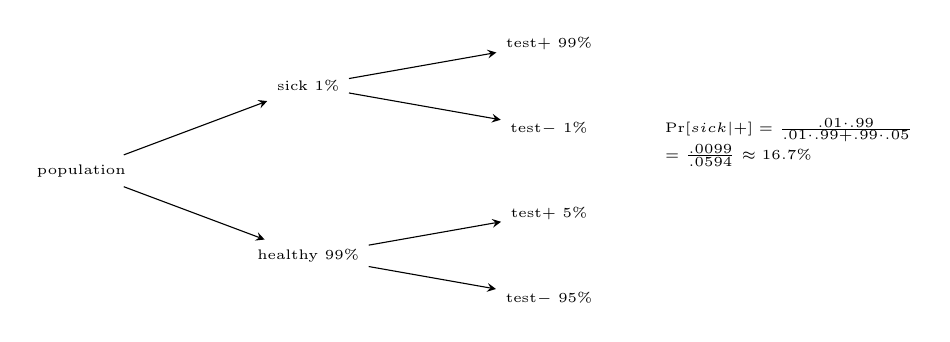
\begin{tikzpicture}[scale=0.9,font=\tiny,grow=right]
\node (r) at (0,1.2) {population};
\node (s) at (3.2,2.4) {sick $1\%$};
\node (h) at (3.2,0) {healthy $99\%$};
\node (pp) at (6.6,3.0) {test$+$ $99\%$};
\node (pn) at (6.6,1.8) {test$-$ $1\%$};
\node (hp) at (6.6,0.6) {test$+$ $5\%$};
\node (hn) at (6.6,-0.6) {test$-$ $95\%$};
\draw[-{stealth}] (r)--(s); \draw[-{stealth}] (r)--(h);
\draw[-{stealth}] (s)--(pp); \draw[-{stealth}] (s)--(pn);
\draw[-{stealth}] (h)--(hp); \draw[-{stealth}] (h)--(hn);
\node[align=left,anchor=west] at (8.1,1.6) {$\Pr[\text{sick}|+]=\frac{.01\cdot.99}{.01\cdot.99+.99\cdot.05}$\\$=\frac{.0099}{.0594}\approx16.7\%$};
\end{tikzpicture}

\caption{Bayes as a renormalised tree. Notice the posterior is
a ratio of two shaded paths: $\Pr[\text{sick}\mid +]$ divides
the sick-and-positive mass by \emph{all} positive mass. Drawing
the tree first prevents the usual denominator mistakes.}
\label{fig:bayes}
\end{figure}

\begin{exercise}[easy] A bag has 3 red and 2 blue marbles; draw
two without replacement. Compute $\Pr[\text{second is red}]$
by total probability over the first draw, and check it equals
$3/5$. Explain the symmetry.\end{exercise}

\section{Distributions as dynamic programs}\label{sec:probdp}
\index{distribution!dynamic programming over}
When the number of steps is large, push the whole distribution
forward one step at a time: a vector of probabilities per state
and a transition that reweights it. Two CSES staples.

\begin{example}[CSES \emph{Throwing Dice}]
Count the number of ways to write $n$ as an ordered sum of
terms in $\{1,\dots,6\}$, modulo $10^9+7$. $n\le 10^{18}$.
\textbf{Strategy.} This is the dice distribution's
denominator: $f(i)=\sum_{j=1}^{6}f(i-j)$. For small $n$ a
sliding six-cell window does it in $O(n)$ --- but the CSES
limit is $n\le 10^{18}$, so the recurrence must be powered as
a $6\times6$ companion matrix (Ch.~14's Fibonacci trick,
extended to a sixth-order recurrence). The state
$[f(i),\dots,f(i-5)]$ advances by one companion-matrix multiply
per step, giving $O(\log n)$.
\end{example}
\begin{solution}
\lstinputlisting{code/throwing_dice.cpp}
Real output on the CSES sample $n=8$:
\begin{verbatim}
125
\end{verbatim}
\end{solution}

\begin{example}[CSES \emph{Moving Robots}]
Each of the $64$ squares of an $8\times8$ board starts with one
robot. Every turn, every robot steps to a uniformly random
neighbouring square. After $k$ turns, print the expected number
of \emph{empty} squares to six decimals. $k\le 100$.
\textbf{Strategy.} Square $s$ is empty iff \emph{no} robot is
there. Robots move independently, and different start squares
stay independent, so for each source robot $t$ run a $k$-step
distribution DP over the board: $p_{t\to s}$ is the probability
$t$'s robot sits on $s$. Then
$\Pr[s\text{ empty}]=\prod_t(1-p_{t\to s})$ and the answer is
$\sum_s$ of that --- linearity again, over 64 vacancy
indicators. (Figure~\ref{fig:robots}.)
\end{example}
\begin{solution}
\lstinputlisting{code/moving_robots.cpp}
Real output on the CSES sample $k=10$:
\begin{verbatim}
23.120740
\end{verbatim}
\end{solution}
\begin{figure}[ht]\centering
\begin{tikzpicture}[scale=0.62,font=\tiny]
\draw[slate,step=1] (0,0) grid (8,8);
\node at (3.5,3.5) {$\frac1d$};
\node at (3.5,2.5) {$d$};
\foreach \p in {(3.5,3.5),(3.5,4.5),(4.5,3.5),(2.5,3.5),(3.5,2.5)}
  \fill[accentsoft] \p circle (6pt);
\node[align=left,anchor=west] at (8.4,4) {each square sends\\$\frac1{\deg}$ of its mass\\to each neighbour\\--- 64 independent\\sources tracked};
\end{tikzpicture}

\caption{One source robot's position distribution after one
turn on the $8\times8$ board --- each neighbour carries mass
$1/\deg$. Notice the vacancy product treats the 64 independent
sources separately; the expectation then sums over squares,
never over robot configurations ($2^{64}$ of them).}
\label{fig:robots}
\end{figure}

\begin{exercise}[medium] In \emph{Moving Robots}, why is
$\prod_t(1-p_{t\to s})$ the correct vacancy probability, and
which step would break if the robots were required to move in
lock-step (all in the same direction)?\end{exercise}

\section{Exact answers vs.\ simulation}\label{sec:sim}
\index{Monte Carlo simulation}\index{precision}
Judges accept answers to $\sim\!10^{-6}$ absolute or relative
error. Two consequences. First, prefer exact arithmetic until
the last moment: probabilities like $7/36$ can be carried as
integer numerator/denominator (with \texttt{\_\_int128} if
needed) and converted once --- or, as in this chapter, kept in
\texttt{double} provided you divide per-step rather than
computing $6^{100}$ first. Second, simulation is a debugging
tool, not a solver: a Monte Carlo estimate with $T$ trials has
error $\Theta(1/\sqrt{T})$, so $10^{12}$ trials buy roughly
$10^{-6}$ --- you cannot get there, and CSES-style six-decimal
acceptance still rejects the variance. Use simulation to
\emph{check} an exact formula, as in the next worked example.

\begin{example}[Coupon collector, exact vs.\ simulated]
For $n$ coupon kinds, compare the closed form $nH(n)$ against
an \texttt{mt19937} simulation of 200{,}000 collectors.
\end{example}
\begin{solution}
\lstinputlisting{code/coupon_collector.cpp}
Real output on $n=6$:
\begin{verbatim}
exact   14.700000
simulated 14.673785
\end{verbatim}
Two hundred thousand trials still miss the second decimal ---
that gap is why simulation verifies and exact DP submits.
\end{solution}
\begin{figure}[ht]\centering
\begin{tikzpicture}[scale=0.85,font=\tiny]
\draw[-{stealth},slate] (0,0)--(7.4,0) node[right]{draws};
\foreach \x/\l in {0/1, 1.2/2, 2.7/3, 4.6/4, 7.0/{5\ldots}}{
  \draw[ink] (\x,0.12)--(\x,-0.12) node[below]{$\l$};}
\foreach \a/\b/\e in {0/1.2/{1}, 1.2/2.7/{6/5}, 2.7/4.6/{6/4}, 4.6/7.0/{6/3}}{
  \draw[decorate,decoration={brace,amplitude=3pt},accent] (\a,0.35)--(\b,0.35)
    node[midway,above=4pt]{$E=\e$};}
\node[align=left] at (3.6,-1.3) {geometric waits: $\frac66+\frac65+\frac64+\frac63+\frac62+\frac61=14.7$};
\end{tikzpicture}

\caption{Coupon collector as a sum of geometric waits. Notice
each stage $i$ waits $\mathbb{E}=1/p_i=n/(n-i)$ draws: the tail stages
($p\to 1/n$) dominate, which is why $H(n)$, not a constant
multiple, appears.}
\label{fig:coupon}
\end{figure}

\begin{exercise}[hard] Prove the tail-sum identity
$\mathbb{E}[X]=\sum_{v\ge1}\Pr[X\ge v]$ for integer $X\ge0$ by
rewriting the double sum $\sum_v\Pr[X=v]\cdot v$ as a triangle
of terms. (Hint: write $v$ as $\sum_{j=1}^{v}1$.)\end{exercise}

\section{Common mistakes}
\index{probability!common mistakes}
\begin{itemize}
\item \textbf{Requiring independence for linearity.}
$\mathbb{E}[X+Y]=\mathbb{E}[X]+\mathbb{E}[Y]$ needs nothing --- the CSES pair-sum and
coupon waits both exploit dependent pieces.
\item \textbf{Adding probabilities of overlapping events.}
$\Pr[A\cup B]$ double-counts $A\cap B$; only add when the
events are disjoint (or use complements/inclusion--exclusion).
\item \textbf{Reaching for \texttt{rand()} early.} Monte Carlo
cannot hit $10^{-6}$ reliably; it belongs in your stress test,
not your submission.
\item \textbf{Precision mistakes at the boundary.} Dividing
\emph{once at the end} by $6^{100}$ overflows; dividing each
step by $6$ is safe. Print with \texttt{\%.6f} from a
\texttt{double}.
\item \textbf{Bayes without the denominator.}
$\Pr[H\mid E]=\Pr[E\mid H]\Pr[H]/\Pr[E]$ and $\Pr[E]$ is a
total-probability sum --- drawing the tree first makes this
mechanical.
\end{itemize}

\section*{Summary}
\begin{tabularx}{\linewidth}{@{}lXl@{}}
\textbf{Need} & \textbf{Tool} & \textbf{Cost}\\
\midrule
``at least one'' & complement rule $1-\Pr[\neg A]$ & $O(1)$\\
P(sum in range) & distribution DP over steps & $O(nS)$\\
expected count & indicators $+$ linearity & one small prob each\\
$E[X]$, $X\ge0$ & tail-sum $\sum\Pr[X\ge v]$ & often closed-form\\
posterior & Bayes with total-prob denominator & tree first\\
many steps, few states & per-source distribution DP & $O(k\cdot|\text{states}|)$\\
sanity-check formula & \texttt{mt19937} simulation & verify only\\
\end{tabularx}

\section*{Exercises}
\begin{exercise}[easy] CSES \emph{Dice Probability} --- re-derive the DP without looking at the listing. \end{exercise}
\begin{exercise}[easy] Two fair dice: compute $\Pr[\text{sum}\ge10]$ by counting, and $\Pr[\text{sum}\ge10\mid \text{first die}\ge4]$ by conditioning. \end{exercise}
\begin{exercise}[easy] Expected value of one fair die, and of the \emph{max} of two fair dice (tail-sum recommended). \end{exercise}
\begin{exercise}[easy] CSES \emph{Throwing Dice} --- implement the sliding window; confirm $f(8)=125$. \end{exercise}
\begin{exercise}[easy] A fair coin until the first head: show the expected number of tosses is $2$ both from the geometric formula and by conditioning on the first toss. \end{exercise}
\begin{exercise}[medium] CSES \emph{Candy Lottery} --- submit the tail-sum solution; then verify $n=2,k=3$ by full enumeration in a script. \end{exercise}
\begin{exercise}[medium] CSES \emph{Inversion Probability} --- implement; derive the closed form $\Pr[x_a>x_b]=\frac{\binom{r_b+1}{2}+(r_a-r_b-1)_+ r_b}{r_a r_b}$ variant when $r_a>r_b$. \end{exercise}
\begin{exercise}[medium] CSES \emph{Moving Robots} --- implement the 64-source DP; check $k=0$ gives $0.000000$ exactly. \end{exercise}
\begin{exercise}[medium] Balls into bins: $m$ uniform balls into $n$ bins; expected occupied bins $=n(1-(1-1/n)^m)$. Prove it with indicators. \end{exercise}
\begin{exercise}[medium] Expected number of tosses of a fair coin to see \emph{two consecutive} heads is $6$ --- derive it by conditioning on the first two outcomes (set up $\mathbb{E}=1+\tfrac12\mathbb{E}[\cdot]$ recurrences). \end{exercise}
\begin{exercise}[medium] CF \emph{Another Problem About Dividing Numbers}-style tasks aside: solve Kattis \emph{Expected Earnings} --- a small direct linearity exercise. \end{exercise}
\begin{exercise}[hard] Expected length of the longest run of heads in $n$ fair flips: derive a distribution DP over (length so far, best so far) and compute it for $n=10$ to six decimals. \end{exercise}
\begin{exercise}[hard] Gambler's ruin: starting with $i$ of $N$ total units, win/lose $\pm1$ each round; prove the expected duration solves a linear recurrence and compute it for $i=N/2$. \end{exercise}
\begin{exercise}[hard] Expected position of the \emph{second largest} of $n$ i.i.d.\ uniform$\{1..k\}$ draws --- generalise the tail-sum approach to the $r$-th order statistic. \end{exercise}
\begin{exercise}[hard] Modular expectation: when a judge asks for $P\cdot Q^{-1}\bmod 10^9+7$, derive why Fermat inversion plus exact counting is exact, and re-implement \emph{Throwing Dice} that way. \end{exercise}

\chapternotes

\section*{Further reading}
\begin{itemize}
\item C.~M.~Grinstead and J.~L.~Snell, \emph{Introduction to
Probability} (2nd ed.) --- free, thorough, finite-sample-space
first; chapters 1, 4 and 6 cover this whole chapter.
(page under:) \newline\url{https://chance.dartmouth.edu/teaching_aids/}
(books\_articles $\to$ probability\_book)
\item MIT OCW 6.041/6.431, \emph{Probabilistic Systems Analysis}
--- full lecture notes and videos; Lectures 1--9 match
\S17.1--\S17.4. (course page under:)
\newline\url{https://ocw.mit.edu/} (courses $\to$ 6-041
Probabilistic Systems, Fall 2010)
\item A.~Laaksonen, \emph{Competitive Programmer's Handbook}
--- the probability chapter; the same CSES problems framed as
contest tools.
\newline\url{https://cses.fi/book/book.pdf}
\item J.~K.~Blitzstein and J.~Hwang, \emph{Introduction to
Probability} (2nd ed.), ISBN 978-1138369917 --- the best
treatment of linearity-without-independence and the indicator
trick anywhere.
\item CSES problem set, \emph{Probability} section ---
eight tasks; five of them are this chapter's worked examples.
\newline\url{https://cses.fi/problemset/}
\item Khan Academy, \emph{Statistics and probability} ---
gentle refresh on expectation and conditioning if the notation
is new.
\newline\url{https://www.khanacademy.org/math/statistics-probability}
\item J.~Pitman, \emph{Probability}, ISBN 978-0387979748 ---
measure-free rigour; where to go when the intuitive arguments
here stop feeling airtight.
\item G.~Grimmett and D.~Welsh, \emph{Probability: An
Introduction} (2nd ed.), ISBN 978-0198574237 --- compact and
proof-first; good second pass after Grinstead--Snell.
\end{itemize}

\begin{rulebox}[Watch instead]
\begin{itemize}
\item \textbf{3Blue1Brown --- ``Bayes theorem, the geometry of
changing beliefs''}, 15m01s,
\url{https://www.youtube.com/watch?v=HZGCoVF3YvM} --- covers
\S17.3: the tree/geometry view that makes the denominator
obvious. Watch this first. (Verified 2026-10-11.)
\item \textbf{MIT OpenCourseWare --- ``1. Probability Models
and Axioms''} (6.041, Tsitsiklis), 51m11s,
\url{https://www.youtube.com/watch?v=j9WZyLZCBzs} --- covers
\S17.1--\S17.3: axioms, conditioning, total probability.
Notation: he writes $P(A^c)$ and $\Omega$ exactly as here.
(Verified 2026-10-11.)
\item \textbf{Khan Academy --- ``Expected Value: E(X)''},
14m53s, \url{https://www.youtube.com/watch?v=j__Kredt7vY} ---
covers \S17.2's definition; note it does \emph{not} prove
linearity for dependent variables, where this chapter's power
comes from. (Verified 2026-10-11.)
\end{itemize}
\emph{Notation note:} all three are discrete-first, matching
this chapter; the OCW lecture additionally uses set-builder
event notation that maps one-to-one onto \S17.1.
\end{rulebox}
The distribution-DP framing follows Laaksonen's probability
chapter and the CSES problem set~\cite{laaksonen2024,cses};
linearity-of-expectation pedagogy follows
Blitzstein--Hwang~\cite{blitzstein2019}; simulation-vs-exact
guidance reflects standard contest practice~\cite{cpalgorithms}.
